


\begin{frame}{Model relaxation description: Intermediate Economic Dispatches (ED-k)}
  % \textbf{If a hypergraph features a partition of \(\cN\) with sparse interconnections (few edges) between subsets, we can remove these edges to solve each subset independently}. To do this, we fix a priori the variables in the removed edges. We search for the optimal values for the fixed variables through an iteratively tightened linear program. \\
  % \vspace{1cm}
  %For instance, in the case of (ED), we leverage the fact that \textbf{the only constraints connecting variables of different days are the storage constraints}:\\
  
  \begin{minipage}[t]{0.45\textwidth}
    \vspace{0cm}
    \begin{figure}
      \begin{tikzpicture}[plane/.style={draw, thick, fill=blue!20, opacity=0.6}, scale = 0.5]
        % Define the number of planes
        \newcommand\NumPlanes{4}
        % Define the distance between planes
        \newcommand\DistPlanes{1.5}
        % Define a list of colors
        \def\colors{{"red", "blue", "green", "orange", "purple"}}
      
        % Draw the planes
        \foreach \i in {0,...,\NumPlanes} {
          % Calculate y-shift based on the plane index
          \pgfmathsetmacro\Shift{\i*\DistPlanes}
          % Draw a plane
          \draw[plane] (0+\Shift,0+\Shift) rectangle ++(3,2);
          % Add a label at the top of each plane
          \node at (1.5+\Shift,2.2+\Shift) {ED-\pgfmathparse{int(\i+1)}\pgfmathresult};
        }
      
        % Connect the corners of the planes
        \foreach \i in {1,...,\NumPlanes} {
          \pgfmathsetmacro\j{\i-1}
          \pgfmathsetmacro\Shift{\i*\DistPlanes}
          \pgfmathsetmacro\PrevShift{\j*\DistPlanes}
          % Retrieve color from list
          \pgfmathsetmacro\Color{\colors[\i-1]}
          % Draw connecting segments
          \draw[thick, \Color] (\PrevShift, \PrevShift) -- (\Shift, \Shift);
          \draw[thick, \Color] (3+\PrevShift, 2+\PrevShift) -- (3+\Shift, 2+\Shift);
        }
      \end{tikzpicture}
        
      
      \caption{(ED) hypergraph representation.}
    \end{figure}
  \end{minipage}
  \begin{minipage}[t]{0.45\textwidth}
    \pause
    \begin{itemize}
      \item We divide the time horizon into \(K\) intervals: 
      \begin{tabular}{l}
         \(\{t_0 \coloneqq 0 ,\ldots, t_1\}\), \pause\\
         \(\{t_1+1,  \ldots, t_2\}\), \pause\\
          \quad \quad \quad\(\ldots\) \pause  \\
         \(\{t_{K-1}+1, \ldots, t_K = T \}\)\pause
      \end{tabular}
      \item We fix a priori the intermediate storage values \(v_{t_k}\) for \(k = 1,\ldots,K\). \pause
      \item We refer to the (ED) problems restricted to each time interval as \textbf{(ED-k)}  \pause 
      \item The corresponding optimal values are \(\mathbf{\cV_{k}(x,v_{t_{k}},v_{t_{k+1},\omega})}\) \pause %this is kind of as saying to the grid, hey you start this storage levels, but must end at this other storage levels
    \end{itemize}
  \end{minipage}
\end{frame}

\begin{frame}{}
  

  \begin{oss}
    \begin{equation}\label{Divided ED eq}
      \cV(x,\omega) = \min_{\{v_{t_k}\}_{k=1}^K}\sum_{k=0}^{K-1}\cV_{k}(x,v_{t_{k}},v_{t_k+1},\omega)
    \end{equation}
  \end{oss}

\end{frame}

\begin{frame}{Model relaxation description: Lower Approximation of (ED)}
  Since each function \(\cV_k\) is piecewise linear convex in \(x,v_{t_K},v_{t_{K+1}}\), it can be approximated by a collection of supporting hyperplanes \(\{\pi^w_{i,k}(x,v_{t_k},v_{t_{k+1}})\}\) of each \(\cV_k\). \\ \pause
  An approximation of (ED) is given by: \pause
  \begin{align*}
    \hat{\mathcal{V}}(x,\omega) & = \min_{\{v_{t_k}\}_{k=1}^K} \sum_{k=0}^K \hat{\mathcal{V}}_k(x,v_{t_k},v_{t_{k+1}}) =                           \\
                                & = \min_{\{v_{t_k}\}_{k=1}^K} \sum_{k=0}^K \theta_{k}^{\omega} \tag{ISP}                                          \\
                                & \quad \quad \text{s.t.} \quad \theta_k^{\omega} \geq \pi_{i,k}^{\omega}(x,v_{t_k},v_{t_{k+1}}) \quad \forall i,k
  \end{align*}
  We refer to this problem as the \textbf{Intermediate Storage Problem (ISP)} \pause
  \\ (I know, very original)

\end{frame}
\begin{frame}{Model description: Relaxed Capacity Expansion(CEP-R)}
  %Thus by substituting \(\cV\) with \( \hat{\cV} \) in (CEP) we obtain the following relaxation:
  \begin{align*}
    \label{CEP-A}
    \min_{x} \; & c'x + \bE_{\omega}\left[\cV(x,\omega)\right] \\  \tag{CEP}
    \text{s.t.} \;     & 0 \leq x_{n,g} \leq X_{n,g}
  \end{align*}
  \pause
  \begin{align*}
    \label{CEP-R}
    \min_{x} \; & c'x + \bE_w\left[\hat{\cV}(x,w)\right] \\  \tag{CEP-R}
    \text{s.t.} \;     & 0 \leq x_{n,g} \leq X_{n,g}
  \end{align*}
  \pause
  Since calculating \( \hat{\cV} \) is straightforward, solving (CEP-R) can be done efficiently with L-shaped or subgradient schemes.
\end{frame}

\section{Decomposition Algorithm}

\begin{frame}{Algorithm}
  % https://q.uiver.app/#q=WzAsMTAsWzEsMCwiXFx0ZXh0e0lucHV0fSJdLFsxLDEsIlxcdGV4dHtSLUNFUH0iXSxbMSwyLCJJU1AoXFxvbWVnYSkgXFw7IFxcZm9yYWxsIFxcb21lZ2FcXGluXFxPbWVnYSJdLFswLDMsIlxcdGV4dHtFRC0xfSJdLFsxLDMsIlxcdGV4dHtFRC0yfSJdLFsyLDMsIlxcZG90cyJdLFszLDMsIlxcdGV4dHtFRC1LfSJdLFsxLDQsIlxcdGV4dHtDb21wdXRlIG5ldyBjdXRzIGZvciB9IFZfayBcXDsgXFxmb3JhbGwgayJdLFs0LDQsIlxcYnVsbGV0Il0sWzEsNSwiXFxoYXR7eF5pfSBcXHRleHR7IGlzIENFUC1vcHRpbWFsfSJdLFswLDFdLFsxLDIsIlxcaGF0e3h9XmkiXSxbMiwzLCJ2X3t0XzB9LHZfe3RfMX0iLDFdLFsyLDQsInZfe3RfMX0sdl97dF8yfSIsMV0sWzIsNV0sWzIsNiwidl97dF97ay0xfX0sdl97dF9rfSIsMV0sWzMsN10sWzQsNywiXFx0ZXh0e0R1YWwgbXVsdGlwbGllcnN9IiwxXSxbNSw3XSxbNiw3XSxbNyw4LCJcXHRleHR7aWYgbmV3IGN1dHN9IiwxXSxbOCwxLCJcXHRleHR7QWRkIGN1dHN9IiwxLHsiY3VydmUiOjV9XSxbNyw5XV0=
  \begin{center}
    \[\begin{tikzcd}[ampersand replacement=\&]
      \& {\text{Input}} \\
      \& {\text{R-CEP}} \\
      \& {ISP(\omega) \; \forall \omega\in\Omega} \\
      {\text{ED-1}} \& {\text{ED-2}} \& \dots \& {\text{ED-K}} \\
      \& {\text{Compute new cuts for } \mathcal{V}_k \; \forall k} \&\&\& \bullet \\
      \& {\hat{x}^i \text{ is CEP-optimal}}
      \arrow[from=1-2, to=2-2]
      \arrow["{\hat{x}^i}", from=2-2, to=3-2]
      \arrow["{v_{t_0},v_{t_1}}"{description}, from=3-2, to=4-1]
      \arrow["{v_{t_1},v_{t_2}}"{description}, from=3-2, to=4-2]
      \arrow[from=3-2, to=4-3]
      \arrow["{v_{t_{k-1}},v_{t_k}}"{description}, from=3-2, to=4-4]
      \arrow[from=4-1, to=5-2]
      \arrow["{\text{Dual multipliers}}"{description}, from=4-2, to=5-2]
      \arrow[from=4-3, to=5-2]
      \arrow[from=4-4, to=5-2]
      \arrow["{\text{if new cuts}}"{description}, from=5-2, to=5-5]
      \arrow["{\text{Add cuts}}"{description}, curve={height=40pt}, from=5-5, to=2-2]
      \arrow[from=5-2, to=6-2]
    \end{tikzcd}\]
  
    % \begin{tikzpicture}[node distance= 1cm]
    %   \node (in) [process] {Input};
    %   \node (rcep) [process, below left=of in] {R-CEP};
    %   \node (isp) [process, below right=of in] {ISP for all \(\omega \in \Omega\)};
    %   \node (ed1) [process, below left=of isp] {ED-1};
    %   \node (ed2) [process, right=of ed1] {ED-2};
    %   \node (edk) [process, right=of ed2] {ED-K};
    %   \node (cuts) [decision, below=of edk] {Compute new cuts for \(V_k\) for all \(k\)};
    %   \node (optimal) [process, below=of cuts] {Optimal cuts in \(\hat{x}^i\) for \(\hat{x}^i\) is CEP-optimal};
    %   \node (duals) [process, below=of cuts] {Dual multipliers};
    %   \node (add) [process, below=of duals] {Add cuts};
    %   \draw[->] (in) -- (rcep);
    %   \draw[->] (rcep) -- (isp);
    %   \draw[->] (isp) -- (ed1);
    %   \draw[->] (ed1) -- (ed2);
    %   \draw[->] (ed2) -- (edk);
    %   \draw[->] (edk) -- node[above] {\(V_{t_k}, V_{t_{k+1}}\)} (cuts);
    %   \draw[->] (cuts) -- (optimal);
    %   \draw[->] (cuts) -- node[above] {new cuts} (duals);
    %   \draw[->] (duals) -- (add);
    %   \draw[->] (add) -- node[above] {new cuts} (cuts);
    %   \draw[->] (add) -- (optimal);
    % \end{tikzpicture}
  \end{center}
\end{frame}


% \begin{frame}{Algorithm}
%   \includegraphics[width = 0.7\linewidth]{Alg.png}
% \end{frame}
% \begin{frame}{Algorithm description} %maybe we can devide this description in the previous slides
%   INPUT: Provide a lower bound for \(\theta_k^{\omega}\) for \(k=1,\ldots,K\) and \( \omega \in \Omega \) and a trial action \(\hat x^0\)
%   \pause
%   \begin{enumerate}[label = {\arabic*}]
%     \item Warm-Start: Calculate initial approximation for \(\mathcal{V}\) for all \(\omega \in \Omega\) around \(\hat{x}^0\). \pause
%     \item For \(i = 1,\ldots,N\): \pause
%           \begin{enumerate}[label = {2.\arabic*}]
%             \item Solve current relaxation (CEP-R) and obtain new trial action \(\hat x^i\). \pause
%             \item For \(\omega \in \Omega \) (in parallel): \pause
%                   \begin{enumerate}[label = {2.1.\arabic*}]
%                     \item Solve the (ISP) approximation problem \(\hat{\mathcal{\cV}}(\hat{x}^{(i)},\omega)\) and obtain intermediate storage values \(\hat{v}^i_k\) for \(k=1,\ldots,K\).\pause
%                     \item Solve (ED-k) (in parallel) for each time step.\pause
%                     \item Using dual multipliers, compute a supporting hyperplane for \(\cV_k\) around \(\hat{x}^i, \hat{v}^i_k, \hat{v}^i_{k+1}\) for \(k=0,\ldots,K-1\).\pause
%                     \item Add the supporting hyperplanes to the approximation problems (ISP) and(CEP-R) \(\hat{\mathcal{V}}(\hat{x}^{(i)},\omega)\).
%                   \end{enumerate}
%           \end{enumerate}
%   \end{enumerate}
% \end{frame}

% \begin{frame}{Algorithm description}
%   INPUT: Provide a lower bound for \(\theta_k^{\omega}\) for \(k=1,\ldots,K\) and \( \omega \in \Omega \) and a trial action \(\hat x^0\)

%   \begin{tabular}{@{}p{0.95\textwidth}}
%     1. Warm-Start: Calculate initial approximation for \(\mathcal{V}\) for all \(w \in \Omega\) around \(\hat{x}^0\). \\
%     2. For \(i = 1,\ldots,N\): \\
%     \quad 2.1. For \(w \in \Omega \) (in parallel): \\
%     \quad\quad\quad 2.1.1. Solve the (ED) approximation problem \(\hat{\mathcal{V}}(\hat{x}^{(i)},\omega)\) and obtain 
%     \\ \quad\quad\quad\quad  intermediate storage values \(\hat{v}^i_k\) for \( k=1,\ldots,K\). \\
%     \quad\quad\quad 2.1.2. Solve (ED) (in parallel) for each time step \(k = 0,\ldots,K-1\),
%     \\ \quad\quad\quad\quad\(V_k(\hat{x}^i,\hat{v}^i_k, \hat{v}^i_{k+1},\omega)\). \\
%     \quad\quad\quad 2.1.3. Using dual multipliers, compute a supporting hyperplane for \(V_k\) around 
%     \\ \quad\quad\quad\quad\(\hat{x}^i, \hat{v}^i_k, \hat{v}^i_{k+1}\) for \(k=0,\ldots,K-1\). \\
%     \quad\quad\quad 2.1.4. Add the supporting hyperplanes to the approximation problem (CEPR)
%     \\ \quad\quad\quad\quad  \(\hat{\mathcal{V}}(\hat{x}^{(i)},\omega)\). \\

%   \end{tabular}
% \end{frame}


\section{Convergence results}
\begin{frame}{Convergence results - 1/5}
  \begin{itemize}
    \item Since \((CEP-R) \leq (CEP)\) if a \((CEP-R)\) optimal solution is (CEP) feasible then it's also \((CEP)\)-optimal. \pause
  \end{itemize}

  \hfill \\


  \textbf{Remark 1:} It is sufficient to prove that after a finite number of steps \((i)\) of the algorithm we have:
  \begin{equation}
    \hat{\cV}(\hat x^i,\omega) = \cV(\hat x^i,\omega)  \text{ for all }  \omega \in \Omega
  \end{equation}


\end{frame}


\begin{frame}{Convergence results - 2/5}
  \begin{oss}
    After a finite number of iterations no new cuts are found for \(\cV_k\).
  \end{oss}
  \begin{proof}
    \begin{align}
       & \uncover<2->{\#\{p \mid p \text{ is a normal vector of a supporting hyperplane of } \mathcal{V}_k\} \leq \nonumber }\uncover<3->{ \\
       & \#\{\text{dual solutions } p=q'B^{-1} \text{ of (ED-k) for varying } x, v_{t_k}, v_{t_{k+1}}\} \leq \nonumber }\uncover<4->{      \\
       & \#\{\text{basis matrices of (ED-k)}\} < \infty }
    \end{align}
    \pause \pause \pause \pause
    After a finite number of steps: \pause
    \begin{itemize}

      \item new cut: \(\bar c (x,v)= \textcolor{deepblue}{p}'(x,v) + b\)  \pause
      \item an old cut: \(\pi(x,v) = \textcolor{deepblue}{p}'(x,v) + \bar b\)

    \end{itemize}


  \end{proof}
\end{frame}


\begin{frame}[noframenumbering]{Convergence results - 3/5}



  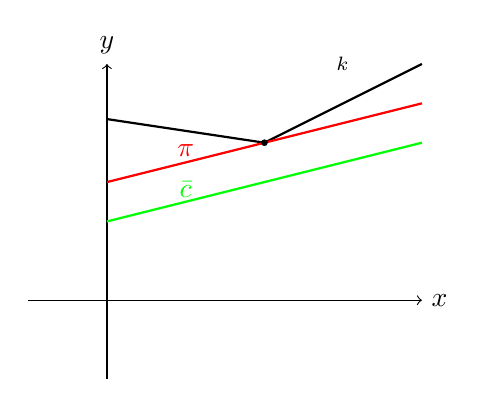
\begin{tikzpicture}[scale=1]
    % Draw axes
    \draw[->] (-1,0) -- (4,0) node[right] {$x$};
    \draw[->] (0,-1) -- (0,3) node[above] {$y$};

    % Define function breakpoints
    \def\xbreak{2}
    \def\ybreak{2}

    % Draw piecewise function
    \draw[thick] (0,2.3) -- (\xbreak,\ybreak);
    \draw[thick] (\xbreak,\ybreak) --  (4,3);

    % Draw tangent line (touching the curve at one point)
    \draw[thick, red] (0,1.5) -- (4,2.5);

    % Mark the touching point
    \filldraw[black] (\xbreak,\ybreak) circle (1pt);

    % Draw parallel line slightly beneath the first one
    \draw[thick, green] (0,1) -- (4,2);

    \draw (3,3) node {$\cV_k$};
    \draw (1,1.90) node[red] {$\pi$};
    \draw (1,1.41) node[green] {$\bar c$};

  \end{tikzpicture}
  \pause
  \\ Since both are supporting hyperplanes it follows that \( b = \bar b\) \\(and therefore \( \bar c\) is not a new cut).
\end{frame}
\begin{frame}{Convergence results - 4/5}
  \begin{oss}
    If after the \(i\)-iteration no new cuts are added for some \(i\) and \(k\) then \(\hat{\cV}_k(\hat x^i, \hat v_{k},\hat v_{k+1}) = \cV_k(\hat x^i, \hat v_{k},\hat v_{k+1}). \) \\ \pause
   
  \end{oss}
  \begin{proof}

    Let \(\bar c_k^{\omega}(x,v_{t_k}) \coloneqq p'(x-\hat x^i, v_{t_k}-\hat v_{t_k}) + \cV_k(\hat x^i,\hat v_{t_k})\) be the new cut found after the \(i\)-th iteration. \\ \pause
    Since \(\bar c\) is not a new cut we have \( \bar c(x,v_{t_k}) \leq \hat\cV_k(x,v_{t_k})\). \pause
    We have thus \[\cV_k(\hat x^i,\hat v_{t_k}) \geq \hat \cV_k(\hat x^i,\hat v_{t_k}) \geq \bar c (\hat x^i,\hat v_{t_k}) = \cV_k(\hat x^i,\hat v_{t_k})\] \pause which concludes the proof.
  \end{proof}

\end{frame}

\begin{frame}{Convergence results - 5/5}
  In conclusion, we have \(\hat{\cV}_k(\hat x^i, v_{t_k},v_{t_{k+1}},\omega) = \cV_k(\hat x^i, v_{t_k},v_{t_{k+1}},\omega)\) for all \(\omega,k\). \pause \\
  Thus \( \hat \cV(\hat x^i,\omega) = \cV(\hat x^i,\omega) \). \pause
  \hfill \\
  \hfill \\
  \begin{prop}
    The algorithm converges after a finite number of iterations and \(\hat x^i\) is an optimal solution for (CEP).
  \end{prop}
\end{frame}

\section{Initial results, Conclusions and Future work}
\begin{frame}{Initial results - 1/2}
  \begin{minipage}[t]{0.45\textwidth}
  We implemented the algorithm on the following network, consisting different kinds of storage units, solar, gas and wind power for a time horizon of 5 weeks and time steps of one hour.
  \end{minipage}
  \begin{minipage}[t]{0.45\textwidth}
  \begin{figure}
    \includegraphics[scale = 0.5]{images/examplenetwork.png}
    \caption{Network layout}
  \end{figure}
  \end{minipage}
 

\end{frame}

\begin{frame}{Initial results - 2/2}
  In this instance the (not parallelized) algorithm converges to the optimal solutions in 12 iterations and in 0.46 seconds. Benders' algorithm converged in 0.44 seconds.
  \begin{figure}
    \includegraphics[scale=0.5]{images/ISPconvergence.png}
    \caption{Objective value of (ISP) for each iteration.}
  \end{figure}
  
\end{frame}

\begin{frame}{Conclusions.}
  \begin{itemize}
  \item The specific structure of the intertemporal constraints makes it possible do develop tailored optimization algorithms for (CEP). \pause
  \item The algorithm is analogous to a three stage bender decomposition. \pause (And I think the work by Filippo Pecci presented yesterday.)
  \end{itemize}
\end{frame}

\begin{frame}{Future Work.}
  \begin{itemize}
    \item We are currently implementing this and other stochastic methods within the Pypsa \cite{PyPSA} framework using the Linopy \cite{Hofmann2023} modeling package in Python. \pause
    \item Supporting hyperplanes for \(\hat{\cV_k(x, v_{t_k}, \omega)}\) could also be used for different \(k' \neq k\) and \(\omega' \neq \omega\), possibly decreasing the overall number of iterations to achieve convergence. \pause
    \item In general: equivalent LP formulations give different corresponding Hypergraph with different degrees of parallelizability.
    %\item Examine generalizations to multistage stochastic programs. \pause
  \end{itemize}

\end{frame}

\begin{frame}
  \vfill
  Thank you for your attention.

  \vfill
  \vfill
  \vfill
  \begin{footnotesize}
    gabor.riccardi01@universitadipavia.it \\
    \url{https://www.compopt.it}
  \end{footnotesize}
\end{frame}
\section{Bibliography}
\appendix
\begin{frame}{}
  Some references:\\[2em]
  \begin{footnotesize}
    \printbibliography[
      %heading=bibintoc,
      title={Bibliography}]
  \end{footnotesize}
\end{frame}

% \begin{frame}[noframenumbering]{Literature}
%   \begin{itemize}
%     \item Traditional stochastic capacity expansion methods, such as the L-shaped method, may perform poorly as the number of expansion possibilities increases.
%    
% \end{frame}



\begin{frame}[noframenumbering]{Power Grid Optimization}
  \begin{itemize}
    \item Optimal Power Flow (OPF) \hfill \textcolor{gray}{\cite{MathProgForm}}
          \begin{itemize}
            \item AC OPF: exact physical model
            \item Security-Constrained OPF (SCOPF) -- Includes contingencies to guarantee system security under failures.
            \item DC OPF and other linearized models \hfill \textcolor{gray}{\cite{LinRelBien} }
            \item other relaxations.
          \end{itemize}

    \item Unit Commitment -- Determines on/off status of power units, ignoring grid constraints.
    \item Economic Dispatch (ED) -- Minimizes generation cost, ignoring grid constraints.
  \end{itemize}
  % Blue arrow on the side of the text
  \begin{tikzpicture}[overlay, remember picture]
    \node at ([shift={(0.9,-1)}]current page.north west) (end0) {}; % Adjust for positioning
    \node at ([shift={(0.9,3)}]current page.south west) (start0) {}; % Adjust for positioning
    \draw[->, thick, blue] (start0) -- (end0) node[midway, fill=white, rotate=90] {Time / Exactness};

    \node at ([shift={(0.3,-1)}]current page.north west) (start1) {}; % Corrected position and syntax
    \node at ([shift={(0.3,3)}]current page.south west) (end1) {}; % Corrected position and syntax
    \draw[->, thick, yellow] (start1) -- (end1) node[midway, fill=white, rotate=90] {Stochasticity}; % Corrected spelling and syntax
  \end{tikzpicture}

  \vfill
  \textbf{Capacity expansion problem:} Based on Economic Dispatch models with added flow balance at bus nodes and various scenarios.
\end{frame}


%possible questions:
% 1) what is the relation between cep-a and the adequacy Assessment?
% Adequacy Assessment span multiple years, over which a certain capability of expanding the grid is expected.
% But the is also ma maximum expected capability to expand thegrid.
% 2) Comparison with L-shaped algorithm (i am a potato)
